% ---------------------------------------------------------------------------- %
\begin{figure}
	\centering
	\subfigure[\label{fig:linguometer:architecture:sig:delay:7}]
	{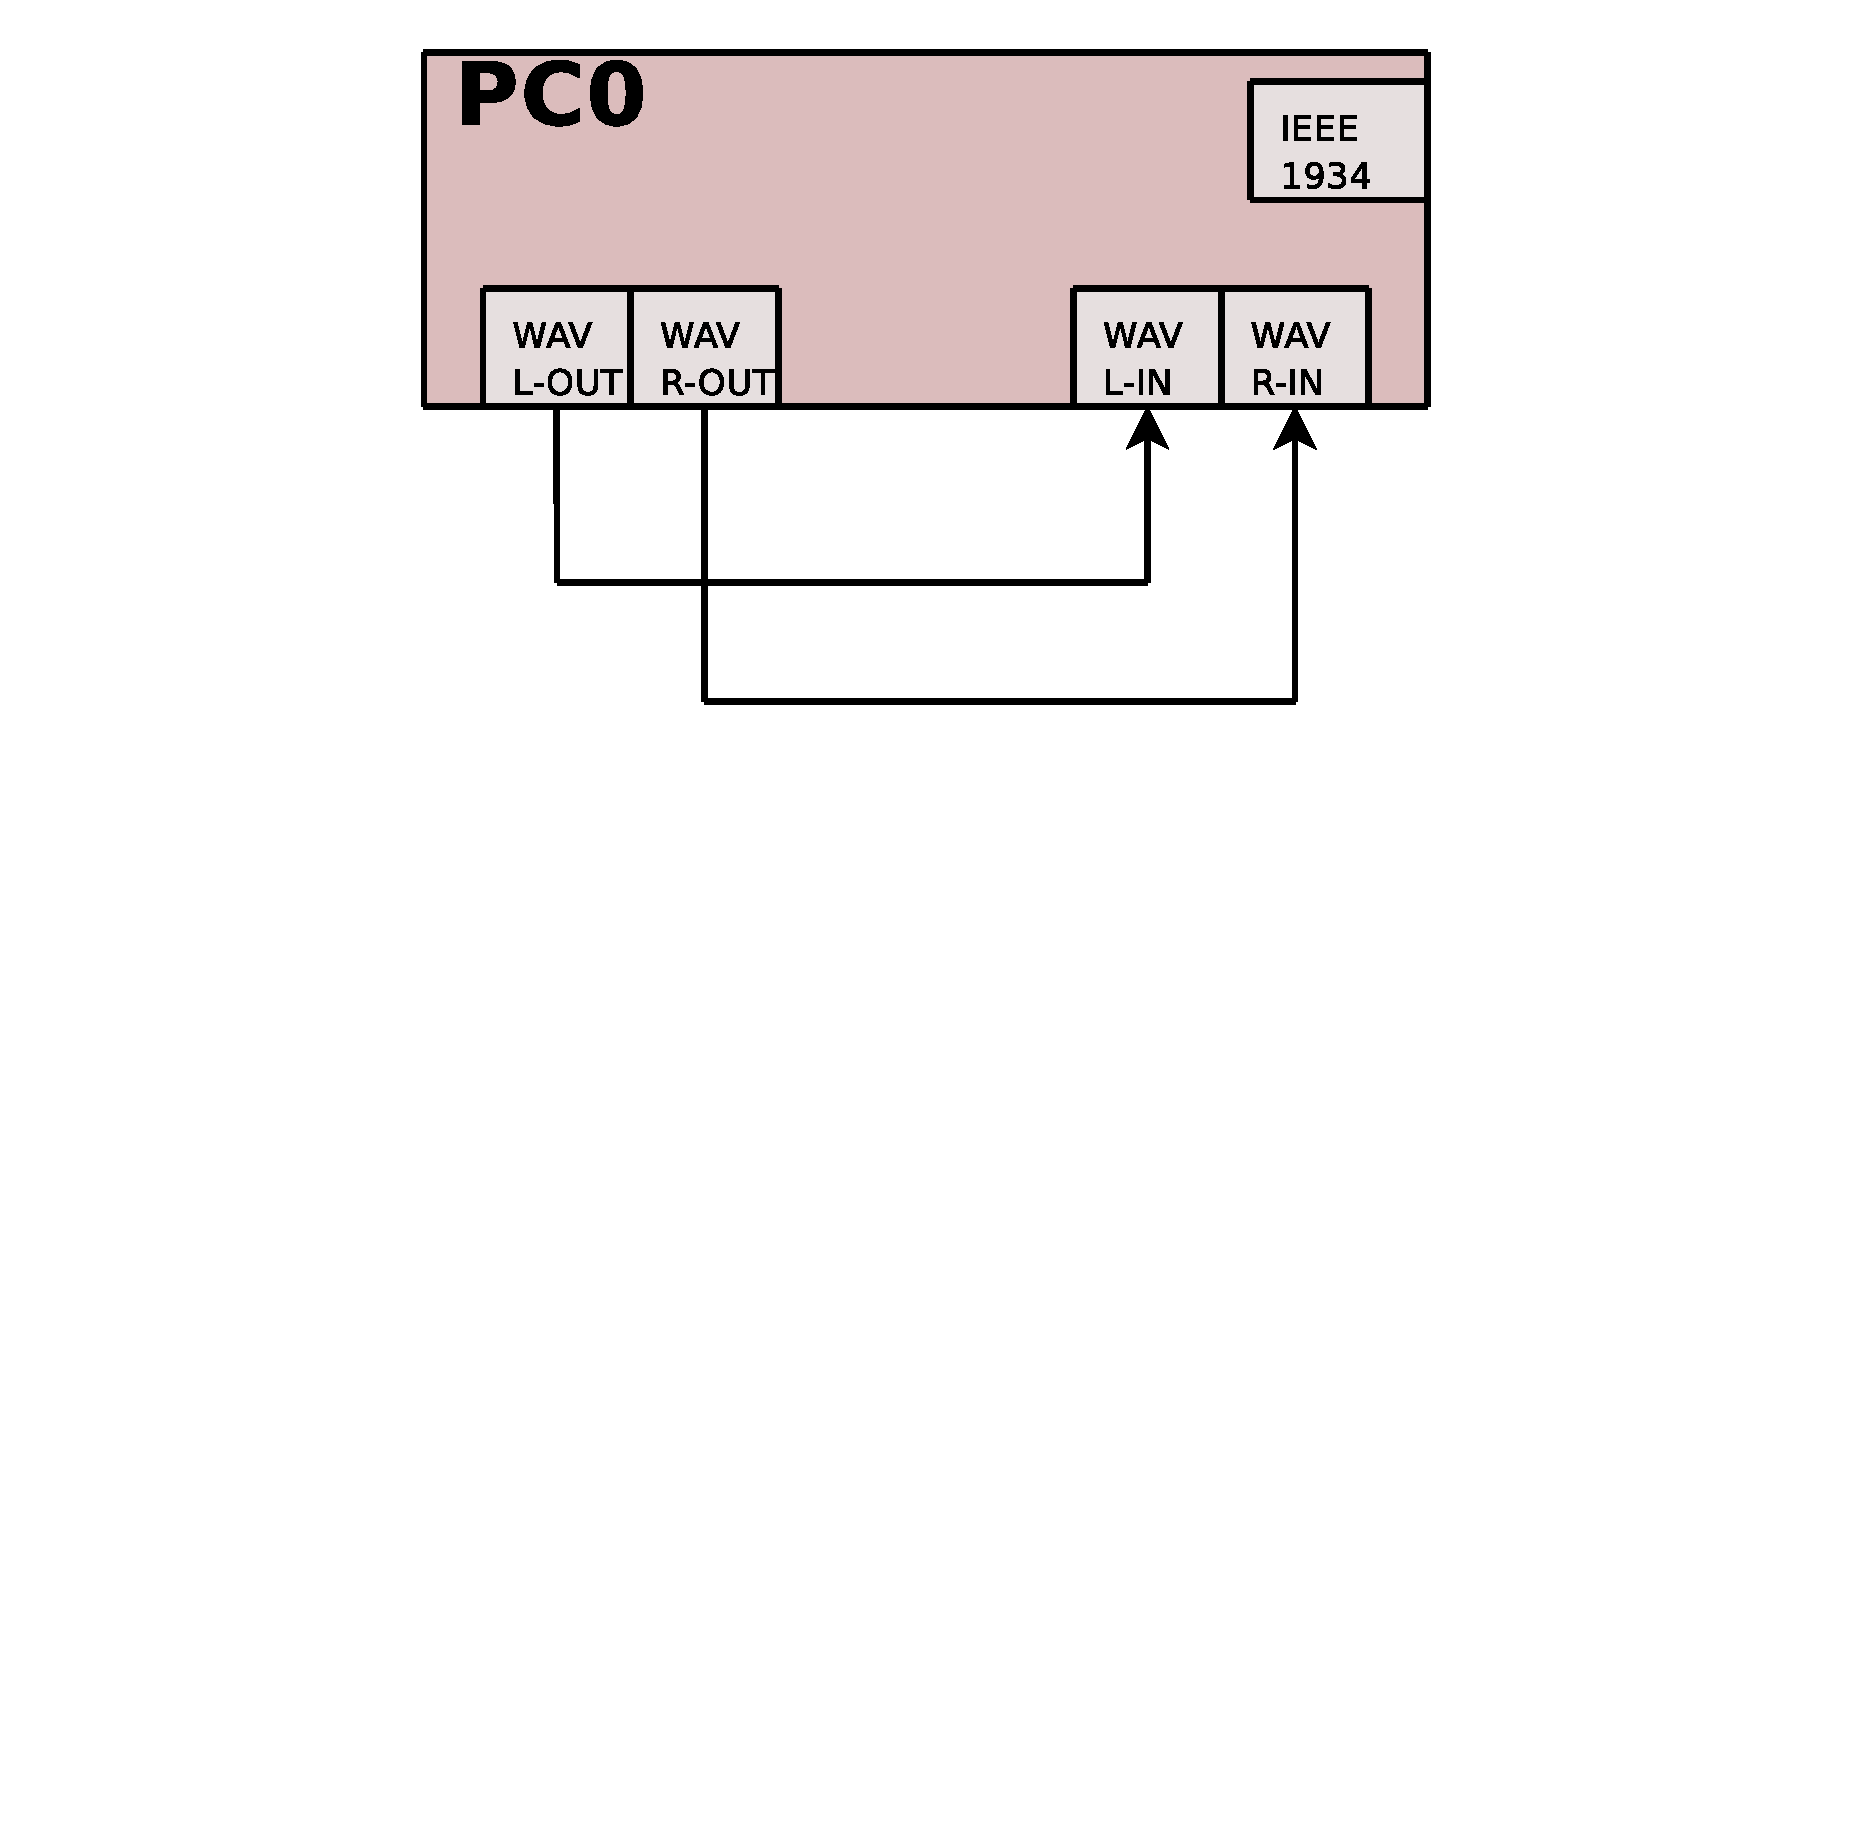
\includegraphics[width=0.32\textwidth]{include/linguometer/images/delay_schemaT.eps}}
	\subfigure[\label{fig:linguometer:architecture:sig:delay:8}]
	{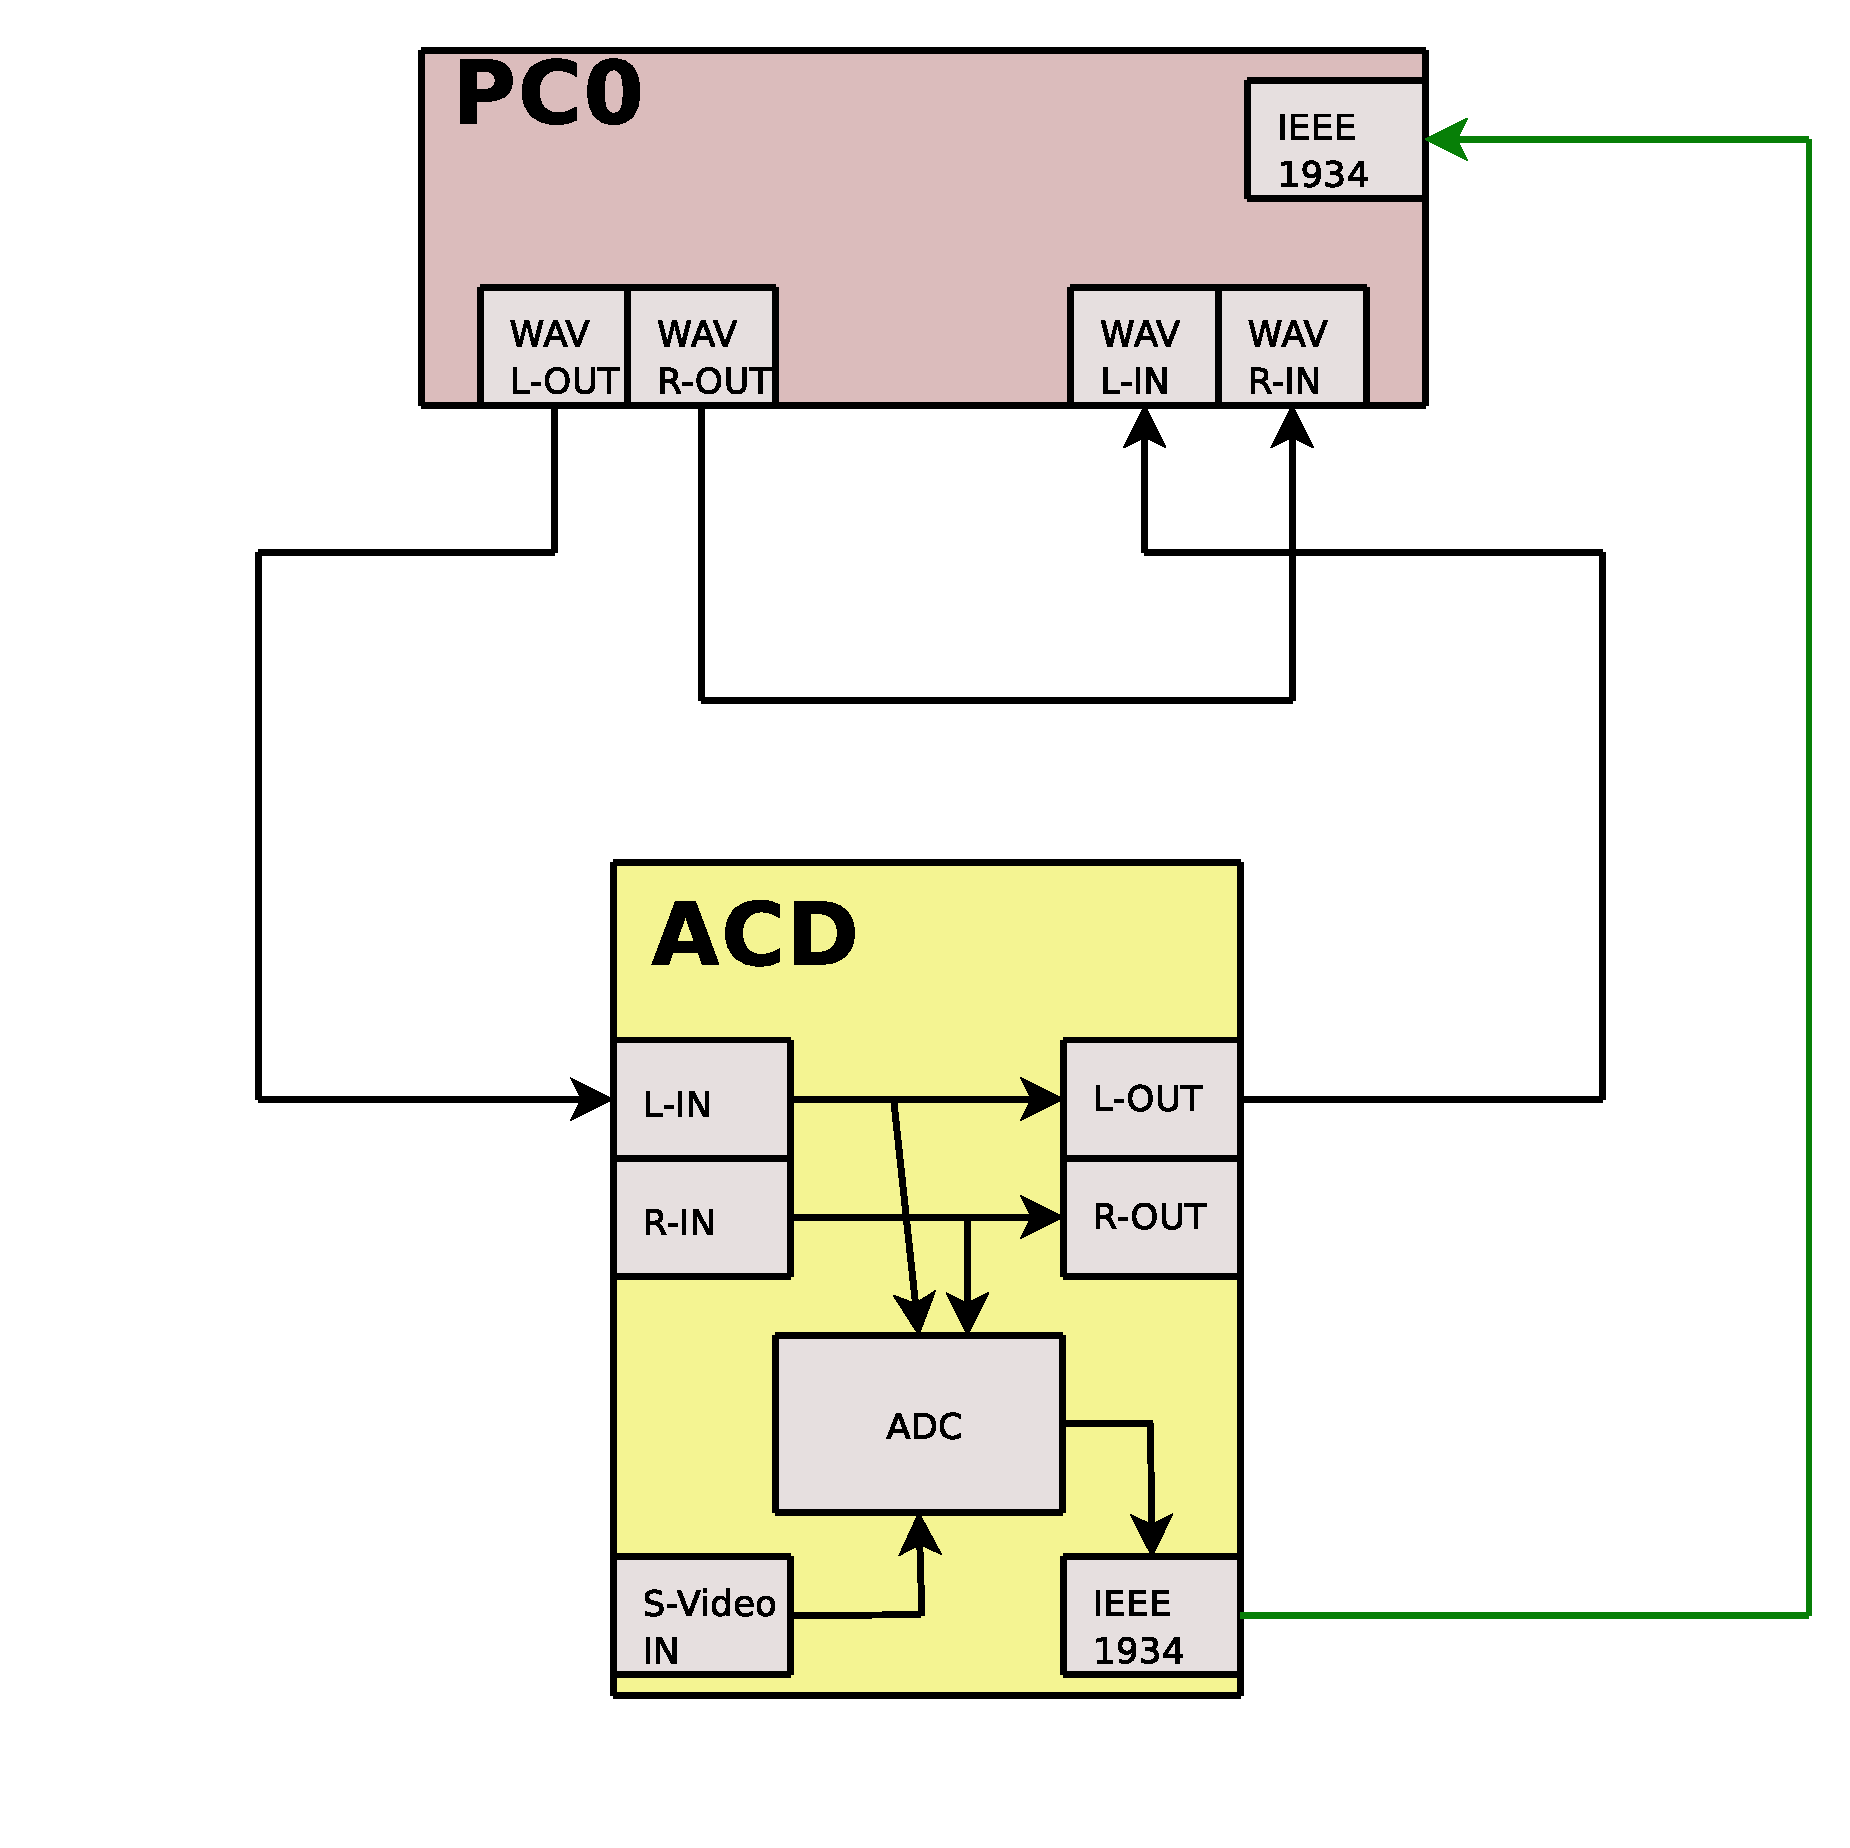
\includegraphics[width=0.32\textwidth]{include/linguometer/images/delay_schemaL.eps}}
	\subfigure[\label{fig:linguometer:architecture:sig:delay:9}]
	{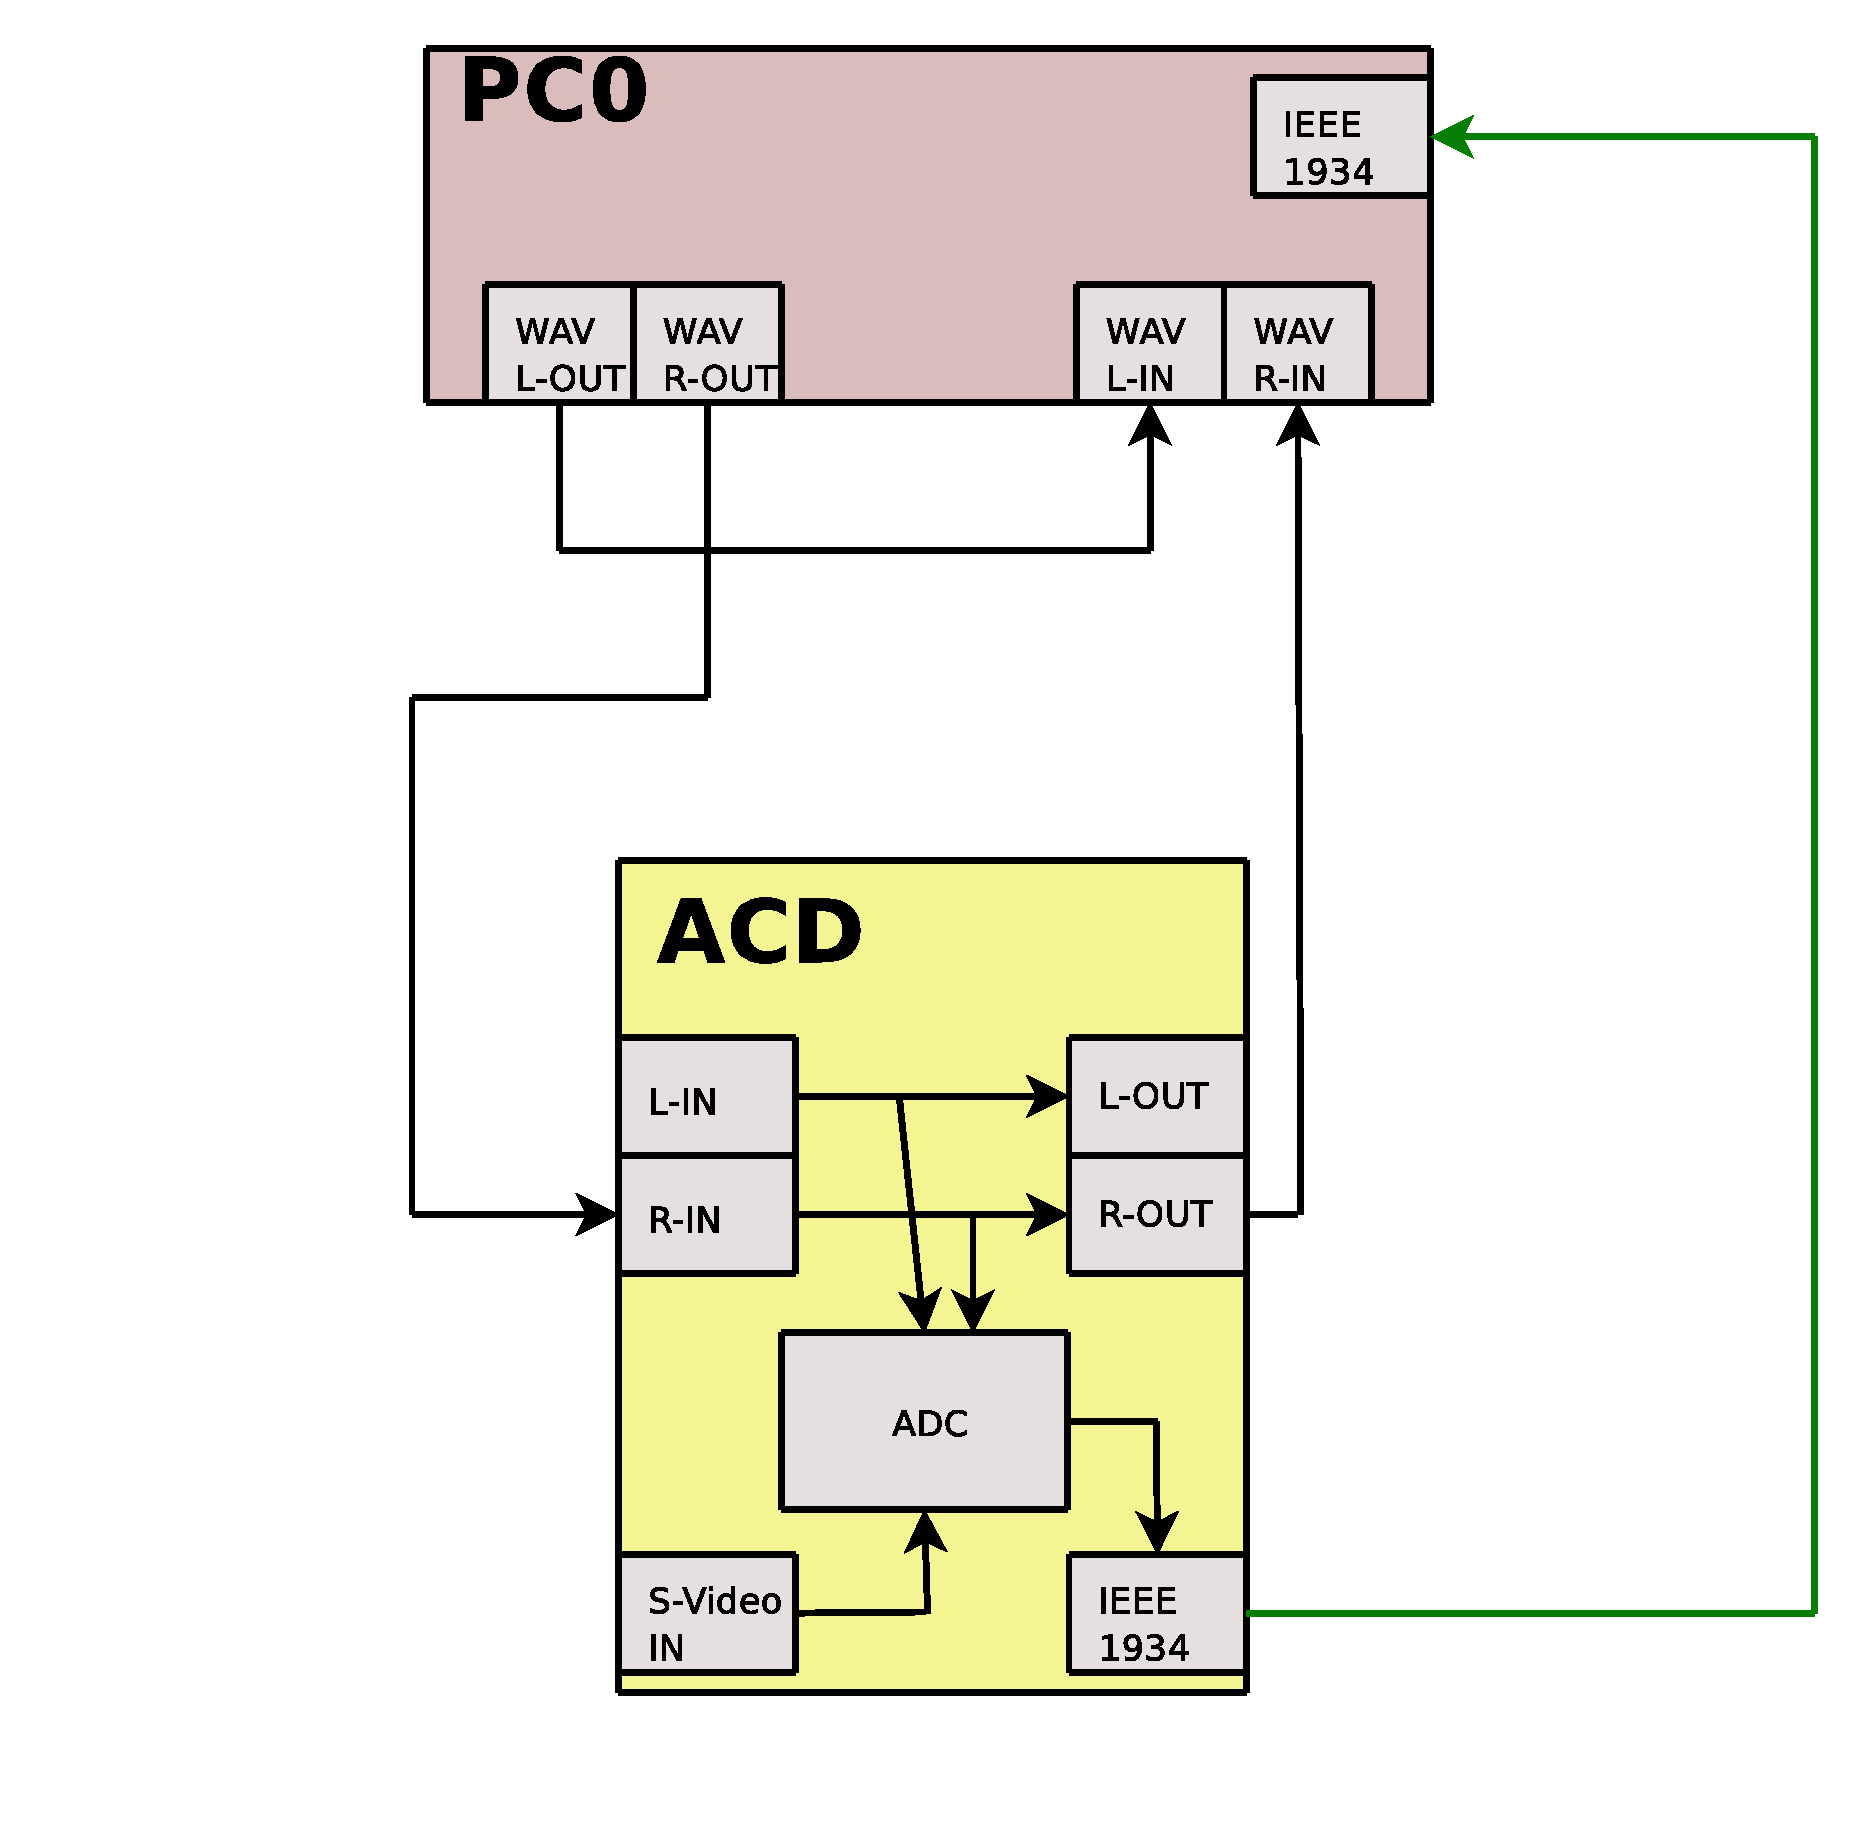
\includegraphics[width=0.32\textwidth]{include/linguometer/images/delay_schemaR.eps}}

	\subfigure[\label{fig:linguometer:architecture:sig:delay:1}]
	{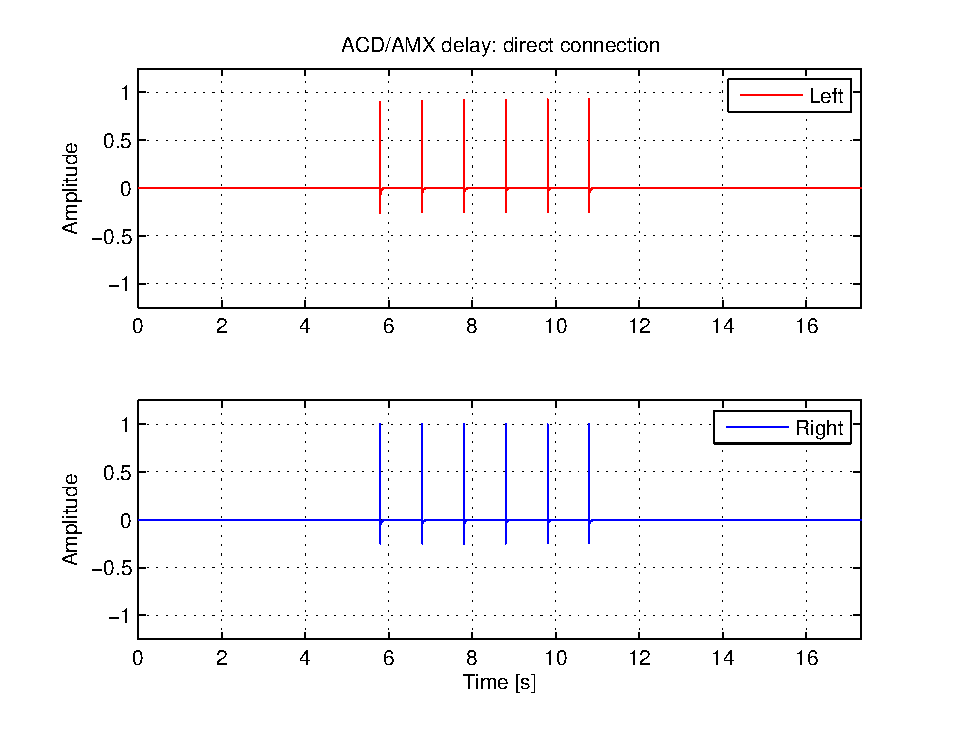
\includegraphics[width=0.32\textwidth]{include/linguometer/images/delay_fullT.eps}}
	\subfigure[\label{fig:linguometer:architecture:sig:delay:2}]
	{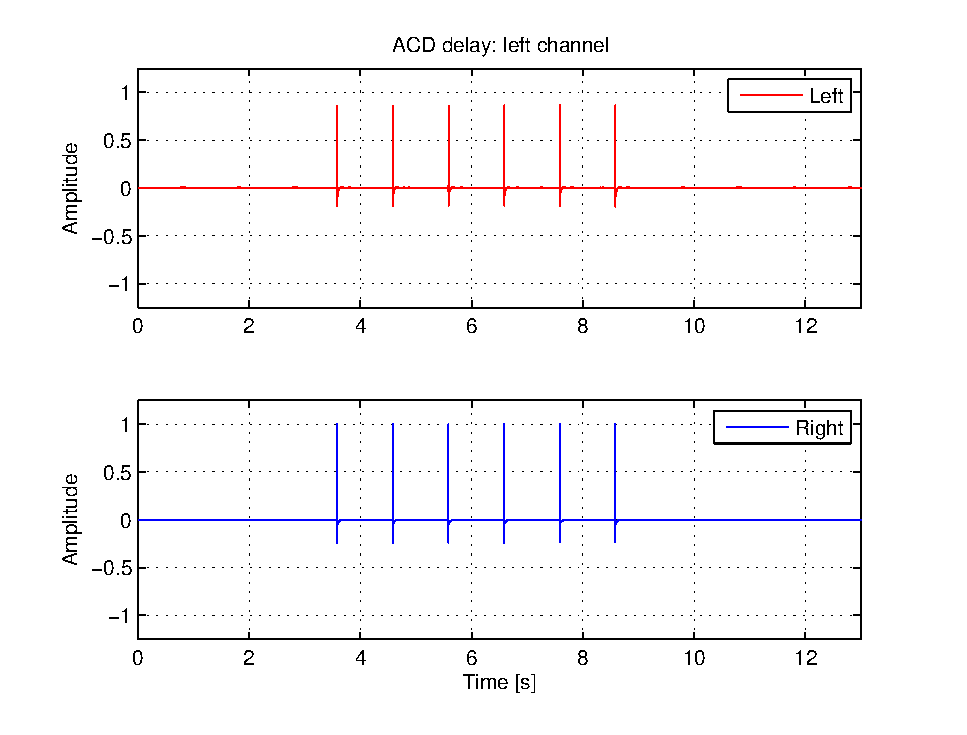
\includegraphics[width=0.32\textwidth]{include/linguometer/images/delay_fullL.eps}}
	\subfigure[\label{fig:linguometer:architecture:sig:delay:3}]
	{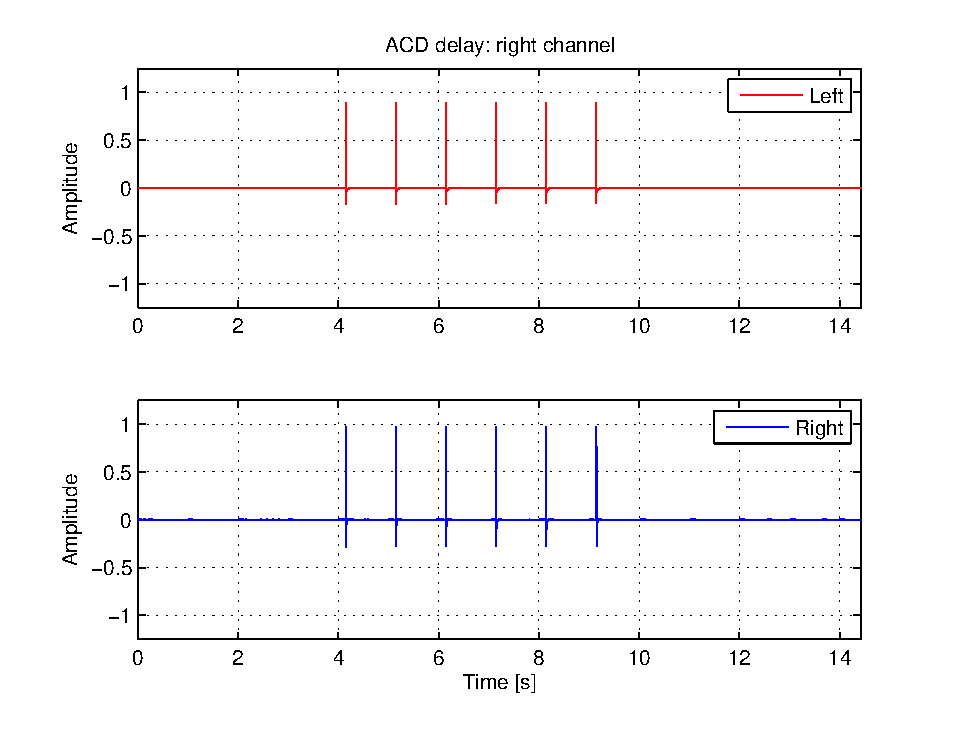
\includegraphics[width=0.32\textwidth]{include/linguometer/images/delay_fullR.eps}}
	
	\subfigure[\label{fig:linguometer:architecture:sig:delay:4}]
	{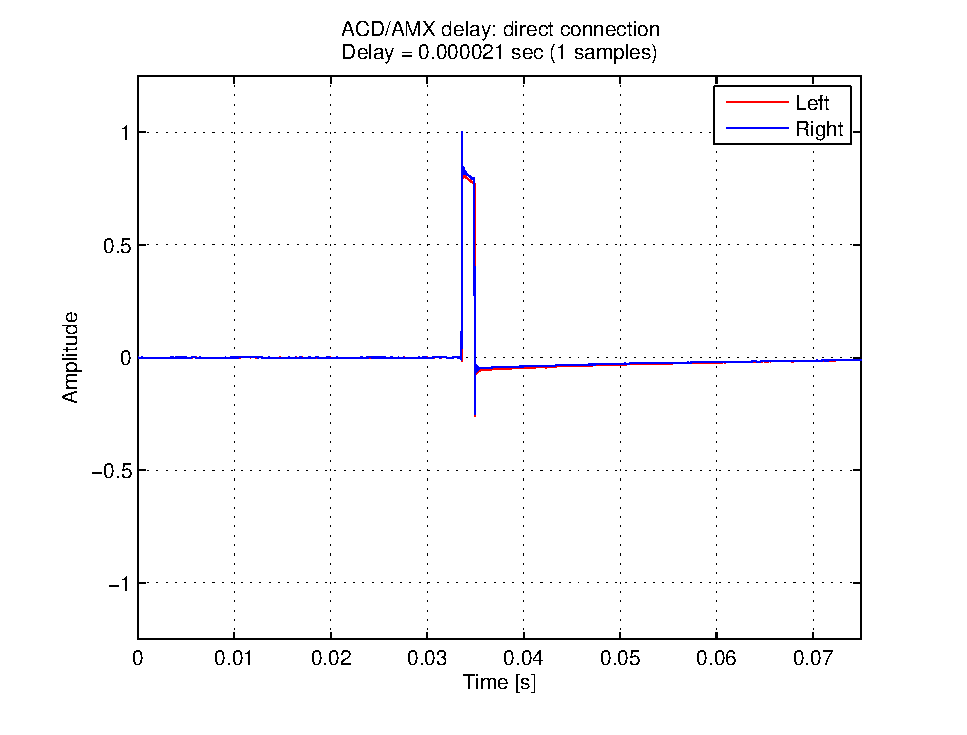
\includegraphics[width=0.32\textwidth]{include/linguometer/images/delay_zoomT.eps}}
	\subfigure[\label{fig:linguometer:architecture:sig:delay:5}]
	{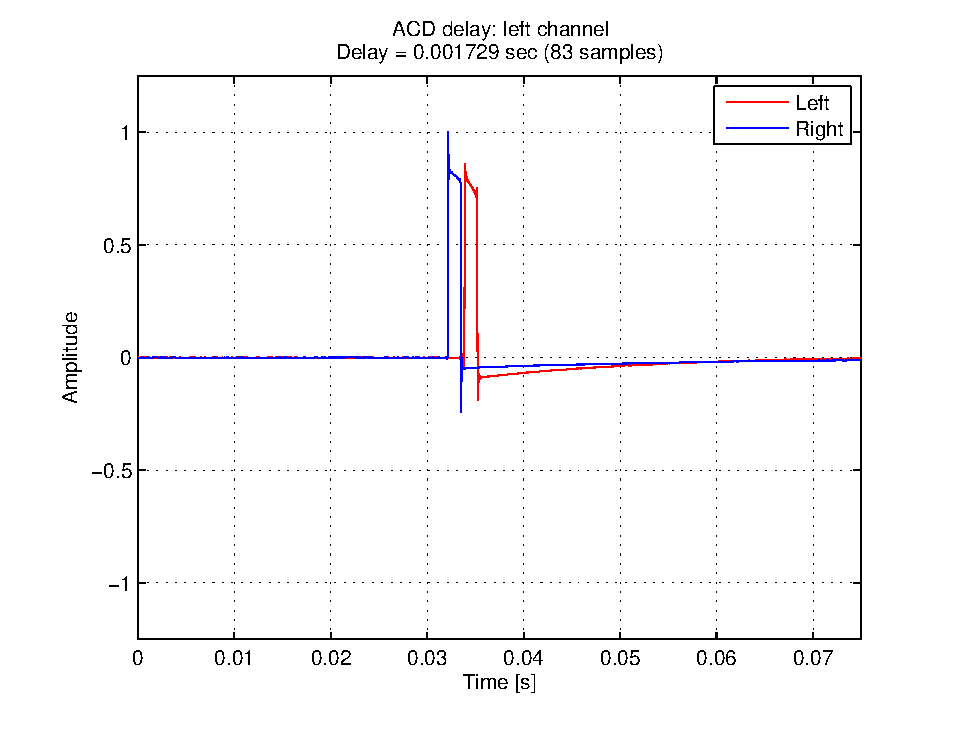
\includegraphics[width=0.32\textwidth]{include/linguometer/images/delay_zoomL.eps}}
	\subfigure[\label{fig:linguometer:architecture:sig:delay:6}]
	{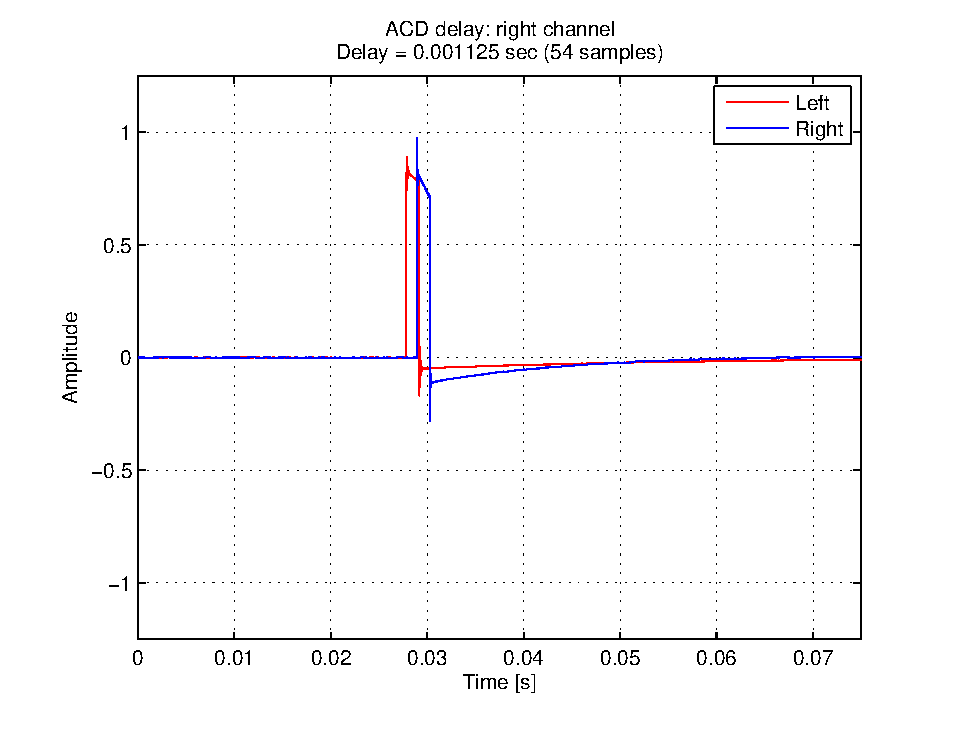
\includegraphics[width=0.32\textwidth]{include/linguometer/images/delay_zoomR.eps}}
	
	\caption[Acquisition card delay]{\textbf{Acquisition card delay}:
	(a) direct connection (reference test);
	(b) left channel trough the delayed device;
	(c) right channel trough the delayed device.
	(d, e, f) Test signals as they are acquired by \sig{PC0}.
	(g, h, i) Firts peak of the acquired signals.
	The plots refer to the first trial.
	}
	\label{fig:linguometer:architecture:sig:delay}
\end{figure}
% ---------------------------------------------------------------------------- %
